\documentclass[singlecolumn]{article}

%%% Some commonly used packages. Feel free to inclued others as needed. %%%
\usepackage[english]{babel}
\usepackage[utf8]{inputenc}
\usepackage{amsmath}
\usepackage{amsfonts}
\usepackage{amssymb}
\usepackage[total={6in, 9in}]{geometry}
\usepackage{graphicx}
\usepackage{hyperref}
\usepackage{subfig}
\usepackage{url}
\usepackage{float}
\graphicspath{ {utils} }


\begin{document}
\title{A Virtual Online Betting System\\
\large Project Report (EE547 Applied and Cloud Computing)}
\author{Hongbo Zhang, Ziyang Zhou, Jiayu Guo}
\date{\today}
\maketitle


\section{Summary}

In this project we built an online platform for users to bet on the NBA games. Every new user will receive 2000 virtual bet points upon registration, which could be placed on the upcoming matches. We will requests odds from well-known online gambling sites via the odds API. After the match ends, users who bet on the winner will get points according to the odds. The betting history will be recorded to users’ profile for them to check. This project contains front-end and back-end. The frontend is deployed on vercel and the backend is deployed on the Railway.app.


\section{Architecture}

Our web application's architecture include 4 parts:
\begin{enumerate}
    \item User: User have a access to login or sign up an account for first time use, and have a betting balance in his account.
    \item Front-End: Interact with user's operation and show the betting webpage to user. Also, send the request to backend and receive response from back End.
    \item Back-End: This is our core part in our project. It will receive request from front-end and give response back to it. It also runs routinely to requests match data from the odds api, and store the fetched data to database.
    \item Database: Provide user's information and provide match information to the back-end, also will record user's information and record match's information from back-end
    \item Odds api: Respond to backend requests. Provide real game information and corresponding odds.
\end{enumerate}

The following sections will present more details on the technologies, implementation and deployment of the architecture.

\begin{figure}[H]
    \centering
    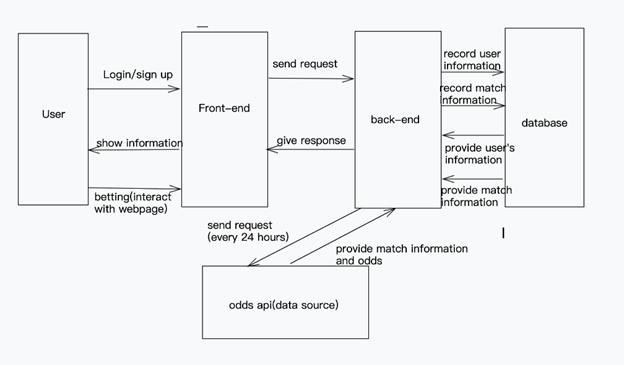
\includegraphics[width=0.8\textwidth]{architecture.png}
    \caption{main architeture of the betting system}
    \label{fig:architecture}
\end{figure}


% \begin{itemize}
% 	\item Predict first-year academic performance without using the rest 2 grades.(Predict G1 without G2 and G3)
% 	\item Predict final-year academic performance without using the rest 2 grades.(Predict G3 without G1 and G2)
% 	\item Predict final-year academic performance using the rest 2 grades as features. (Predict G3 with G1 and G2)
% \end{itemize}

\section{Technologies}
\subsection{Next.js and React}

Next.js is a JavaScript framework that allows you to build server-rendered and statically-generated applications using React. React is a popular JavaScript library for building user interfaces. Next.js and React are commonly used together to build front-end applications because they make it easy to create fast and scalable applications with a simple and intuitive API. Next.js also provides features like automatic code splitting and optimized performance out of the box, making it a great choice for building high-performance front-end applications.

\subsection{Typescript}
TypeScript is a strongly typed, object-oriented, compiled programming language that builds on JavaScript. It is a superset of the JavaScript language, designed to give you better tooling at any scale.


TypeScript may be used to develop JavaScript applications for both client-side and server-side execution (as with Node.js or Deno). Multiple options are available for transpilation. The default TypeScript Compiler can be used, or the Babel compiler can be invoked to convert TypeScript to JavaScript.

\subsection{Tailwind}
Tailwind CSS is a utility-based low-level CSS framework designed to simplify building with speed and less focus on writing custom CSS for web applications.

\subsection{Strapi and graphql}
Strapi is an open-source headless content management system (CMS) that is built on top of Node.js and is used to manage content and make it available through APIs. It allows developers to easily create and manage content types and their fields, as well as define and manage relationships between different types of content.

Strapi supports multiple databases including SQLite, MongoDB, MySQL, and Postgres, and APIs such as RESTful and graphql. In our implementation, we chose the SQLite as database and graphql as API. Additionally, Strapi is highly customizable, allowing us to extend its capabilities and integrate it with the external datasources.


\section{Pages}
Figure \ref{fig:pages} below illustrates the main pages and their relationships in our project. 

\begin{figure}[H]
    \centering
    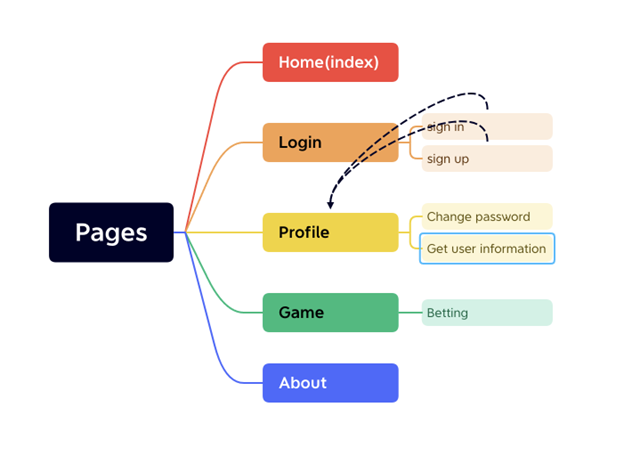
\includegraphics[width=0.9\textwidth]{pages.png}
    \caption{chart illustrating the pages and their relations}
    \label{fig:pages}
\end{figure}


\section{Implementation}

\subsection{Front end}

We use the home page to provide some information about matches. These data are real information obtained from the NBA API every day.

\subsubsection{Home page}

\begin{figure}[H]
    \centering
    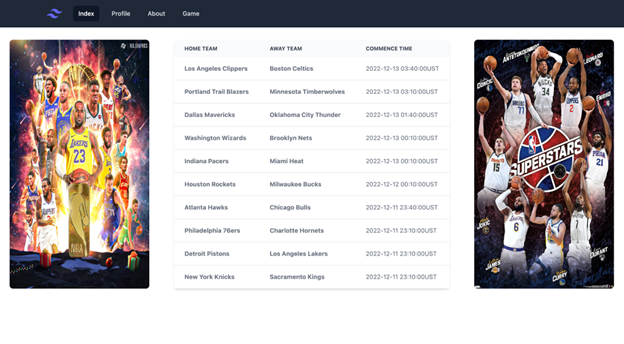
\includegraphics[width=0.6\textwidth]{index.png}
    \caption{index page}
    \label{fig:index}
\end{figure}

Here is core code:

\begin{figure}[H]
    \centering
    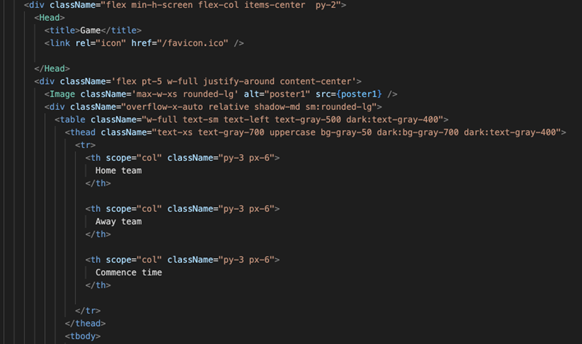
\includegraphics[width=0.6\textwidth]{index_code.png}
    \caption{index core code}
    \label{fig:index_code}
\end{figure}

\subsubsection{Login}
We have 3 features related to user account handling: register, log in, and change password. 

For sign in, if the username does not exist, no changes will be made to this page. If the password is wrong, there will be a corresponding prompt. The sign up page asks you to re-enter your password in case you make a mistake. 

\begin{figure}[H]
    \centering
    \begin{minipage}[c]{0.3\textwidth}
    \centering
    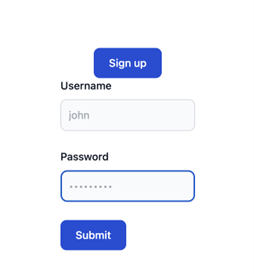
\includegraphics[width=0.9\textwidth]{sign.png}
    \end{minipage}%
    \begin{minipage}[c]{0.3\textwidth}
    \centering
    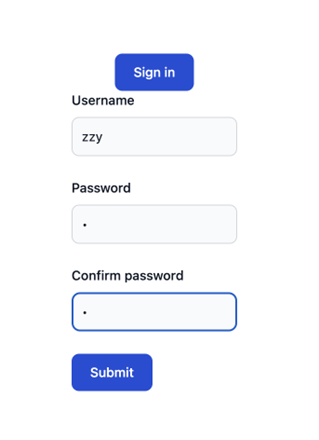
\includegraphics[width=0.9\textwidth]{sign_up.png}
    \end{minipage}%
    \begin{minipage}[c]{0.3\textwidth}
    \centering
    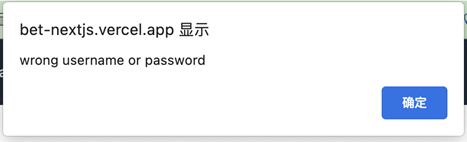
\includegraphics[width=0.9\textwidth]{wrong_sign.png}
    \end{minipage}
    \caption{content definitions}
\end{figure}

The password could also be changed when user enter his profile page.

\begin{figure}[H]
    \centering
    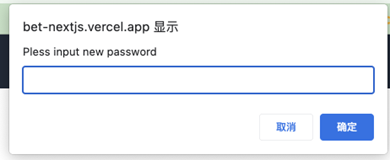
\includegraphics[width=0.6\textwidth]{change_password.png}
    \caption{change password}
\end{figure}

Here is some core code:

\begin{figure}[H]
    \centering
    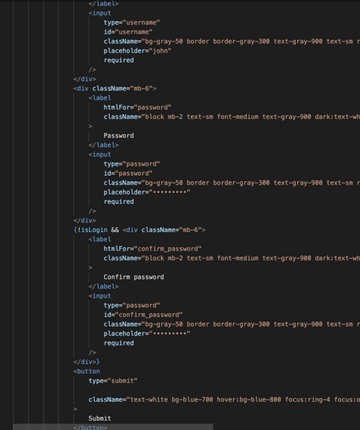
\includegraphics[width=0.6\textwidth]{sign_code1.png}
    \caption{sign page HTML code}
\end{figure}

\begin{figure}[H]
    \centering
    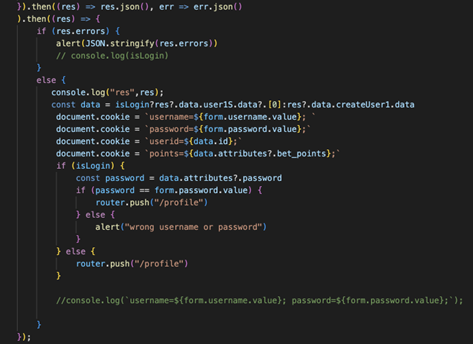
\includegraphics[width=0.6\textwidth]{sign_code2.png}
    \caption{Jump to profile page}
\end{figure}

\subsubsection{Profile}
Once the user create a new account or successfully login, the web page will automatically jump to the profile interface. New users will have 2000 initial bet points. If the user has already logged in, the user could also click the button in the upper left corner of the page to jump to this page. The profile page have the function of logging out and changing the password. It uses graphql to query the user information and the associate history bet records.

\begin{figure}[H]
    \centering
    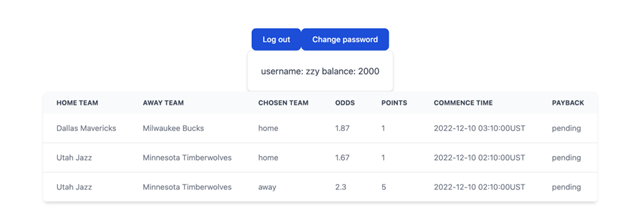
\includegraphics[width=0.6\textwidth]{profile.png}
    \caption{Profile page}
\end{figure}

\begin{figure}[H]
    \centering
    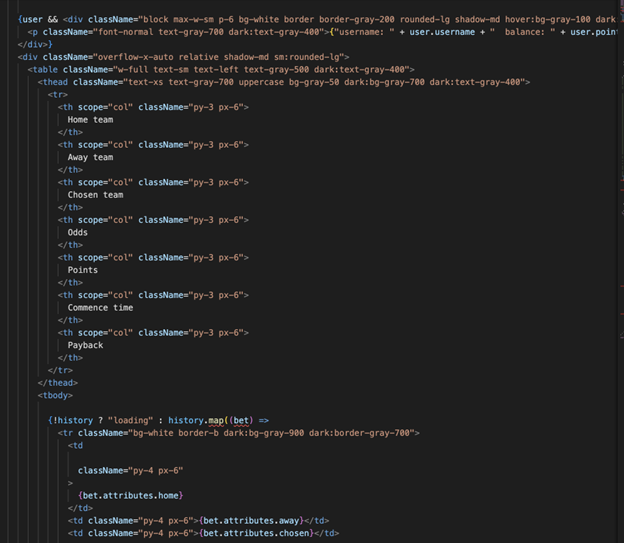
\includegraphics[width=0.6\textwidth]{profile_code.png}
    \caption{Profile core code}
\end{figure}

\subsubsection{Game}

After logging in, users can place bets on the Game tab. There are different games to choose from in the interface. After choosing a team, users can choose how much to bet on. When the bet is successful committed, there will be a message reminding the bet. The process of this part of data use graphql api to query the available bets and corresponding match information.

\begin{figure}[H]
    \centering
    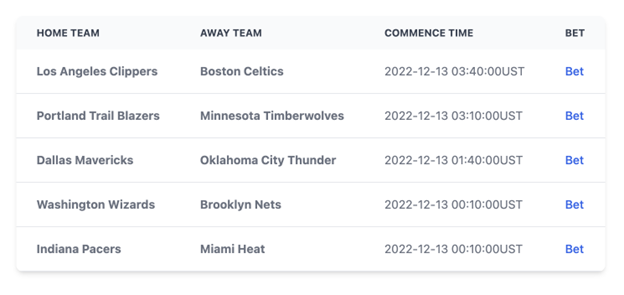
\includegraphics[width=0.6\textwidth]{bet1.png}
    \caption{available bets}
\end{figure}

\begin{figure}[H]
    \centering
    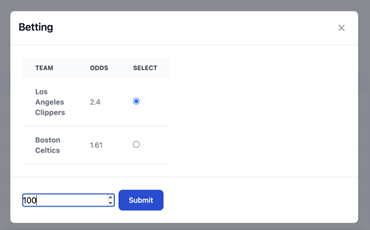
\includegraphics[width=0.6\textwidth]{bet2.png}
    \caption{betting page}
\end{figure}

\begin{figure}[H]
    \centering
    
\includegraphics[width=0.6\textwidth]{bet3.png}
    \caption{successful bet response}
\end{figure}

\subsection{Backend and database}

\subsubsection{Database schema}


We use the SQLite, the default database setting of strapi, to store our user and match data. There are 3 main collections in our database: available bets, users and bets. The schema is shown in the following table. It is built using strapi's content builder. Notice that every available bet (match) has a UID which relates matches to bet record. The bet record also has an one to one relation to an exact user.


\begin{figure}[H]
    \centering
    \begin{minipage}[c]{0.3\textwidth}
    \centering
    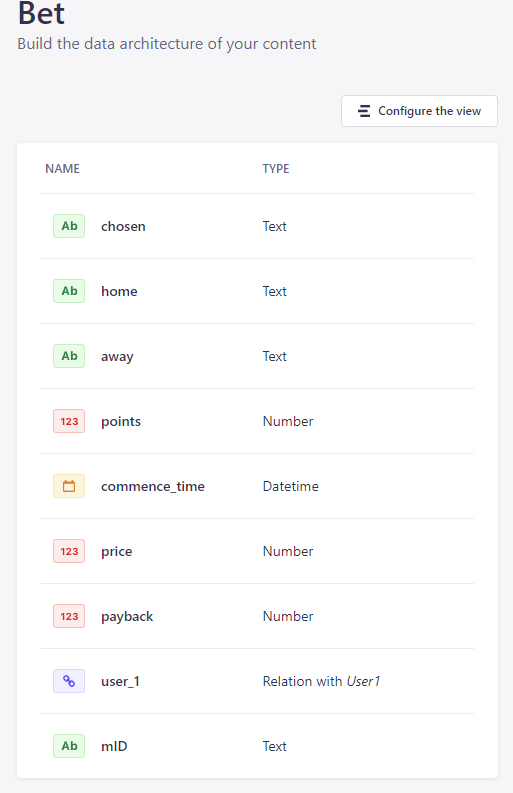
\includegraphics[width=0.9\textwidth]{BetSchema.png}
    \end{minipage}%
    \begin{minipage}[c]{0.3\textwidth}
    \centering
    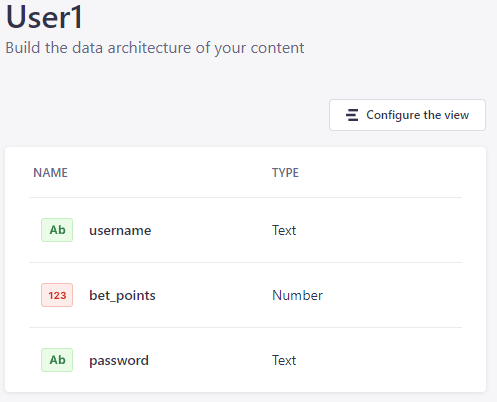
\includegraphics[width=0.9\textwidth]{user1Schema.png}
    \end{minipage}%
    \begin{minipage}[c]{0.3\textwidth}
    \centering
    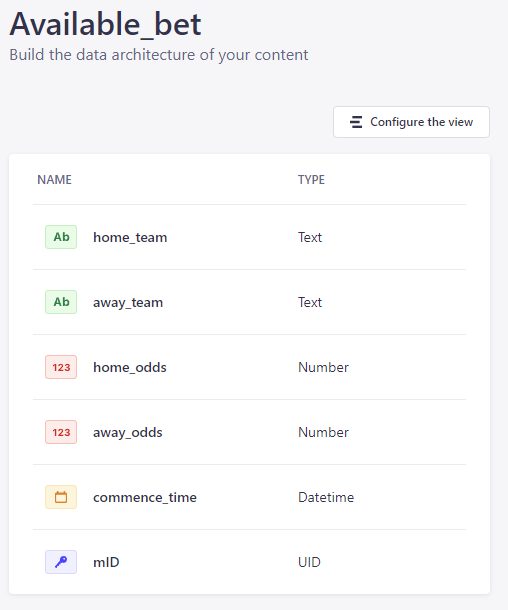
\includegraphics[width=0.9\textwidth]{available_betSchema.png}
    \end{minipage}
    \caption{sign pages}
\end{figure}


\subsubsection{External API usage and data manipulation}

We use axios to requests match data and odds via the odds api. Since the odds api limit the maximum requests to 500 per month in the free tier, we set the match update and bet settlement interval to 24 hours. 

The requested match information includes home and away teams, commence time and the home and away odds. We requests the decimal odds. For example, 1.5 means users will get 150 points back including an initial 100 points betted. 2 cron tasks were set to handle the match creation and bet settlement. The code are shown in the figures below.

\begin{figure}[H]
    \centering
    \begin{minipage}[c]{0.5\textwidth}
    \centering
    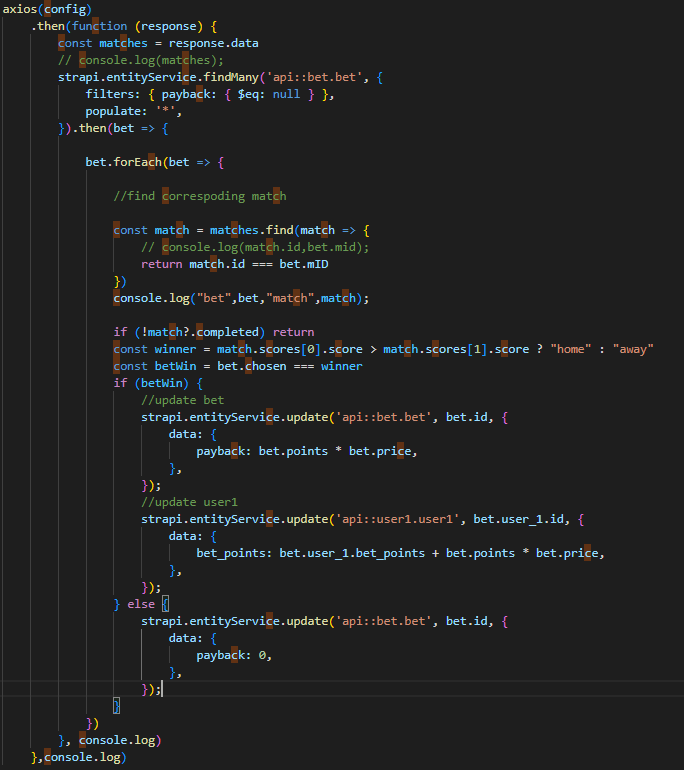
\includegraphics[width=0.9\textwidth]{cron1.png}
    \end{minipage}%
    \begin{minipage}[c]{0.5\textwidth}
    \centering
    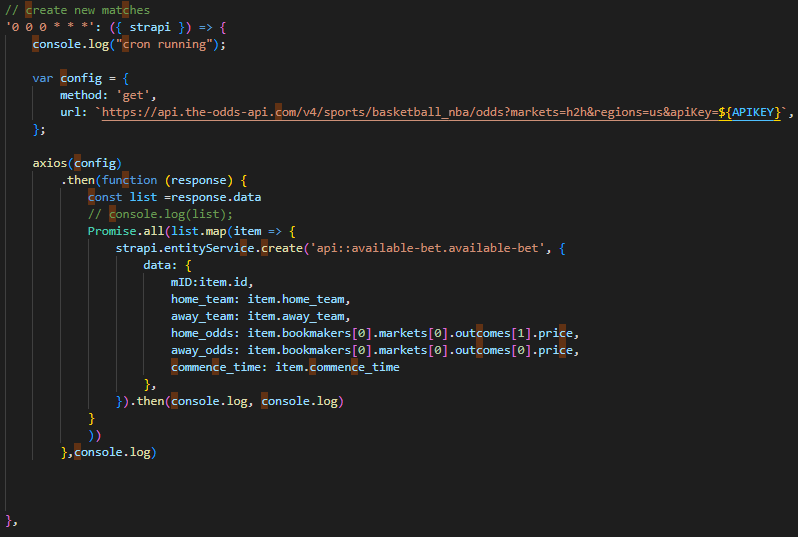
\includegraphics[width=0.9\textwidth]{cron2.png}
    \end{minipage}%
    \caption{code for the cron tasks}
\end{figure}


\subsubsection{Graphql API}

By default Strapi create REST endpoints for each of our content-types. With the GraphQL plugin, we managed to add a GraphQL endpoint to fetch and mutate our content. Strapi uses a Shadow CRUD to automatically generates the type definitions, queries, mutations and resolvers based on the data model defined in the previous section. However, some of our data needs to be protected from the frontend for the sake of security. So I disabled some of the CRUD operations to avoid data leak or illegal mutations.The core code are shown in below figure.

\begin{figure}[H]
    \centering
    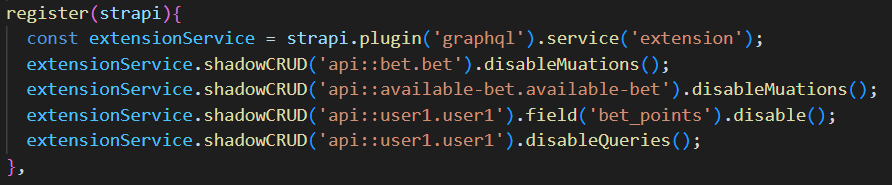
\includegraphics[width=0.6\textwidth]{disable_CRUD.png}
    \caption{Code to disable some endpoints}
\end{figure}


The main graphql schema, queries and mutations are listed in the below figures.

\begin{figure}[H]
    \centering
    \begin{minipage}[c]{0.25\textwidth}
    \centering
    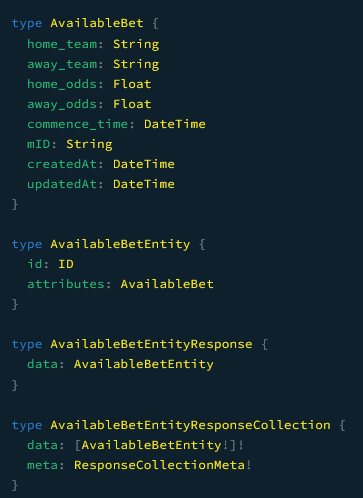
\includegraphics[width=0.9\textwidth]{graphqlschema1.png}
    \end{minipage}%
    \begin{minipage}[c]{0.25\textwidth}
    \centering
    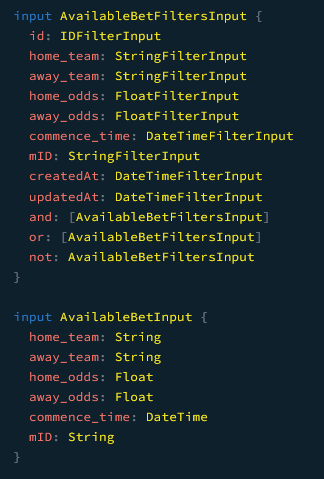
\includegraphics[width=0.9\textwidth]{graphqlschema2.png}
    \end{minipage}%
    \centering
    \begin{minipage}[c]{0.25\textwidth}
    \centering
    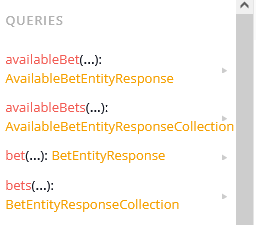
\includegraphics[width=0.9\textwidth]{graphql1.png}
    \end{minipage}%
    \begin{minipage}[c]{0.25\textwidth}
    \centering
    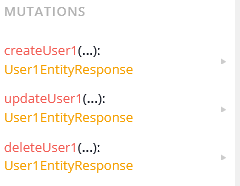
\includegraphics[width=0.9\textwidth]{graphql2.png}
    \end{minipage}%
    \caption{Graphql endpoints}
\end{figure}

\subsubsection{New bet process}

Although strapi provides customization and overites on schema and resolvers. We didn't managed to successfully develop a working graphql resolver for the new bet records created by the users. So instead we use a special RESTful API for the newly created bets. The API code is shown below. If a bet is created before the commence time and user have enough bet points, the bet record will be created. Otherwise the backend wont edit the database and emits an error message.

\section{Cloud Deployment}
The cloud deployment consists of 2 parts. The frontend is deployed on vercel. The backend and the database are deployed together on the Railway App. Both 2 platforms provides auto-generated domain name, which saved us a lot of time in domain configuration.

\subsection{Cloud provider and instance types}
Vercel is a cloud platform for hosting websites and web applications, providing easy and fast deployment of applications built with React and Next.js. 

Railway is another cloud deployment platform which provides simple and efficient deployment from local code base. Railway also offers a consumption-based pricing model, making the cost negligible. The backend and database are deployed on an elastic virtual machine which has at most 512MB RAM, 2vCPUs and 1GB disk, which is sufficient to handle large scale user bet activities and match updates. The figure \ref{fig:resource} shows the of the compute resource usage.



\begin{figure}[H]
    \centering
    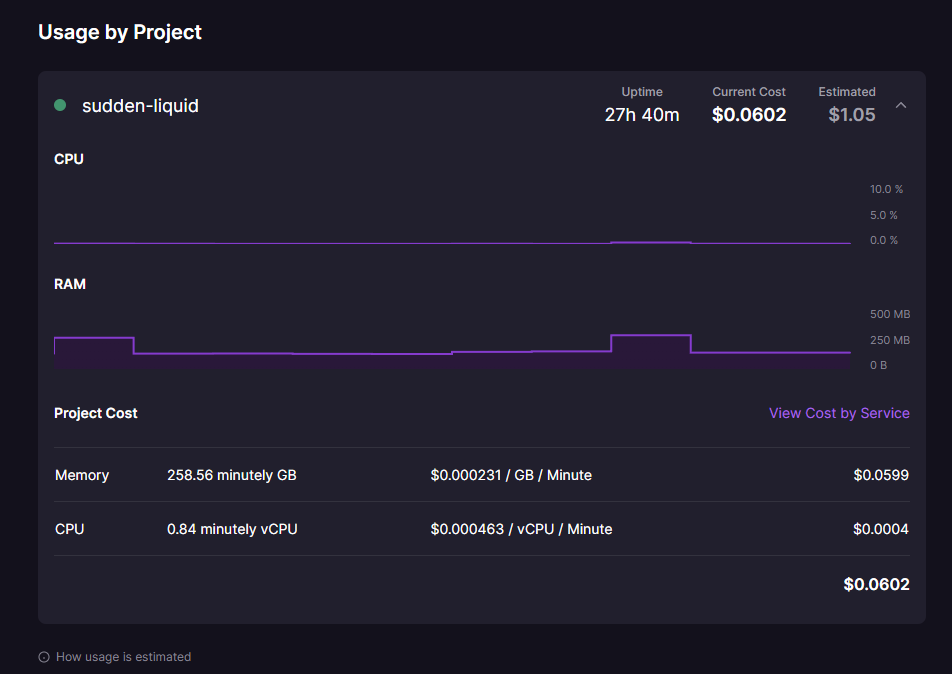
\includegraphics[width=0.6\textwidth]{resource.png}
    \caption{compute resource usage}
    \label{fig:resource}
\end{figure}

\section{Problems and Difficulties}

We initially planend to use the NBA api to get the match information. The NBA api could provide more abundant information including history winning rate of a certain team. However, the NBA api could not be used on the cloud server since the api author banned those ips. So we changed to requests those information from the odds api, which functions well after deployment. We also encountered some difficulties
in customize the graphql resolver in the strapi framework, as mentioned in the previous section. 

\section{References}

\begin{enumerate}
    \item https://nextjs.org/
    \item https://reactjs.org/docs/handling-events.html
    \item https://tailwindcss.com/
    \item https://www.youtube.com/watch?v=mTz0GXj8NN0 (next.js)
    \item https://strapi.io/
    \item https://the-odds-api.com/
    \item https://vercel.com/docs
    \item https://docs.railway.app/
    \item https://axios-http.com/docs/intro
    \item https://en.wikipedia.org/wiki/Cron
\end{enumerate}







\section{Team Roles}

    Hongbo Zhang: Back-end and deployment

	Ziyang Zhou: Front-end

	Jiayu Guo: Responsible for front-end and back-end communication


\end{document}

% --------------------------------------------- TEMPLATES ---------------------------------------------%
%\begin{equation}
%\label{eq:label}
%L(s) = \frac{8}{s(s^2 + 6s + 12)}
%\end{equation}

%\begin{figure}[h]
%	\centering
%	\includegraphics[width = \columnwidth]{image.extension}
%	\caption{Figure caption.}
%	\label{fig:label}
%\end{figure}


%\begin{table}[h]
%\caption{Table caption. \label{tab:label}}
%\centering
%	\begin{tabular}{ c | c | c | c }
%		${\mathbf \tau_z}$ & {\bf \% O.S.} & {\bf Rise time} & {\bf Settling time (2\%)}\\ \hline
%		0 & 32.7 & $9.81.10^{-2}$ & 0.892\\ \hline
%		0.05 & 4.54 & $9.59.10^{-2}$ & 0.387\\	\hline
%		0.1 & 0 & $7.47.10^{-2}$ & 0.489\\	\hline
%		0.5 & 29.2 & $2.55.10^{-2}$ & 1.05
%	\end{tabular}
%\end{table}